\documentclass[pdftex,11pt]{article}
\usepackage[pdftex]{graphicx}
\usepackage{enumerate}
\usepackage{amsmath}
\usepackage{amssymb}
\usepackage{multicol}
\usepackage{algpseudocode}
\usepackage{algorithm}
\usepackage{hyperref}
\usepackage{ listings}
\title{COMP 540 - Homework 4}
\author{Guangyuan Yu(gy12),I still don't have a teammate}
\date{6 March 2017}
\begin{document}
\maketitle


\section{Kernelizing the k-nearest neighbors}
The distance we use in k-nn is
\begin{equation}
dis(x^{(i)},x^{(j)})=(x^{(i)},x^{(j)})^{2}=x^{(i)}*x^{(i)}-2*x^{(i)}*x^{(j)}+x^{(j)}*x^{(j)}
\end{equation}
We can kernelize the distance using Gaussian kernel K, which satisfies the Mercer Condition
\begin{equation}
\begin{split}
dis(x^{(i)},x^{(j)})=&exp(-\frac{||x^{(i)}-x^{(i)}||}{2\sigma^{2}})-2*exp(-\frac{||x^{(i)}-x^{(j)}||}{2\sigma^{2}})+exp(-\frac{||x^{(j)}-x^{(j)}||}{2\sigma^{2}})\\
=&2-2-exp(-\frac{||x^{(i)}-x^{(j)}||}{2\sigma^{2}})
\end{split}
\end{equation}
\section{Constructing kernels}
\subsection{}
For arbitrary \{$x_{1},x_{2}...x_{n}$\} and $g\in R^{n}$, we show that 
\begin{equation}
g^{'}Kg=\sum_{i,j}g_{i}K(x_{i},x_{j})g_{j}=\sum_{i,j}g_{i}c*k_{1}(x_{i},x_{j})g_{j}=c*\sum_{i,j}g_{i}k_{1}(x_{i},x_{j})g_{j}\geqslant0
\end{equation}
\subsection{}
\begin{equation}
g^{'}Kg=\sum_{i,j}g_{i}f(x_{i})k_{1}(x_{i},x_{j})f(x_{j})g_{j}=\sum_{i,j}h_{i}k_{1}(x_{i},x_{j})h_{j}\geqslant0
\end{equation}
The last line follows because $k_{1}$ is a kernel function.
\subsection{}
\begin{equation}
g^{'}Kg=\sum_{i,j}g_{i}K(x_{i},x_{j})g_{j}=\sum_{i,j}g_{i}(k_{1}(x_{i},x_{j})+k_{2}(x_{i},x_{j}))g_{j}=\sum_{i,j}g_{i}k_{1}(x_{i},x_{j})g_{j}+\sum_{i,j}g_{i}k_{2}(x_{i},x_{j})g_{j}\geqslant0
\end{equation}

\section{Fitting an SVM classifier by hand}
\subsection{}
we have $x=(0,-1)\rightarrow x=(1,0,0)$ and $x=(\sqrt{2},1)\rightarrow x=(1,2,2)$.\
$\theta^{'}=(0,2,2)$ is parallel to the optimal vector.
\subsection{}
The margin is $\sqrt{2}$. The midpoint is (1,1,1). Margin is also the distance between SV to the midpoint.
\subsection{}
Since $\frac{1}{|\theta|}=\sqrt{2}$, let assume the$ \theta=(0,b,b)$, so that $\frac{1}{\sqrt{2*b^{2}}}=\sqrt{2}$ we get $b=0.5$. $ \theta=(0,0.5,0.5)$
\subsection{}
\begin{equation}
\begin{cases}
-1((1,0,0)*(0,0.5,0.5)+\theta_{0}) & \geqslant1\\
1*((1,2,2)*(0,0.5,0.5)+\theta_{0}) & \geqslant1
\end{cases}
\end{equation}
$\theta_{0}=-1$
\subsection{}
\begin{equation}
(0,1/2,1/2)*(1,\sqrt{2}x,x^{2})-1=0
\end{equation}
\begin{equation}
\frac{\sqrt{2}x}{2}+\frac{x^{2}}{2}-1=0
\end{equation}
\section{Support vector machines for binary classification}


\subsection{The hinge loss function and gradient}
From Jupyter, I get $J =  1.0  grad =  [-0.12956186 -0.00167647]$\\
The code is 
\begin{lstlisting}
  correctness = y * X.dot(theta)
  J = 1. / (2 * m) * sum(theta ** 2) + 1. * C / m * sum(1 - correctness[correctness < 1])
  grad = 1. / m * theta + 1. * C / m * (-y[correctness < 1].dot(X[correctness < 1]))
  return J,grad
\end{lstlisting}
\subsection{impact of varying C}
\begin{figure}[H]
  \caption{Example dataset 1}
  \centering
    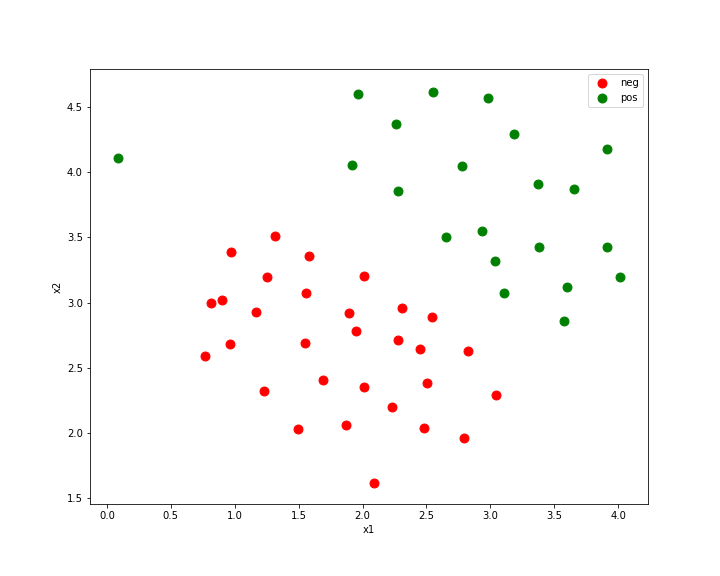
\includegraphics[scale=0.5]{oridata.png}
\end{figure}

\begin{figure}[H]
  \caption{C=100}
  \centering
    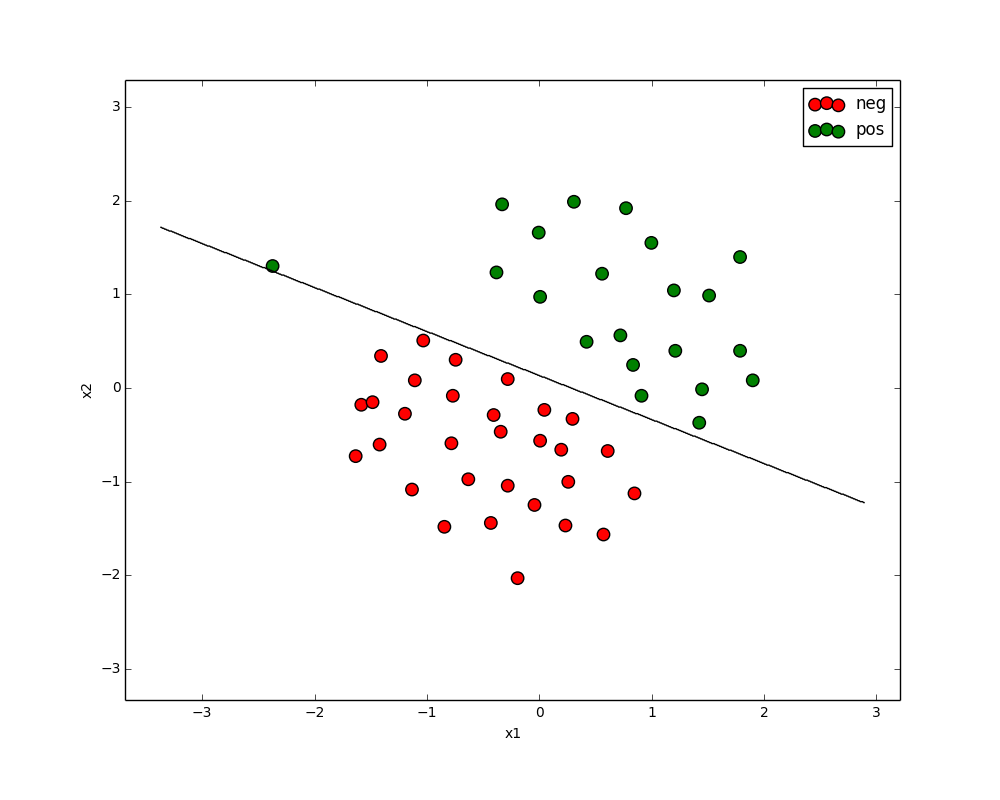
\includegraphics[scale=0.5]{c100.png}
\end{figure}

\begin{figure}[H]
  \caption{C=10}
  \centering
    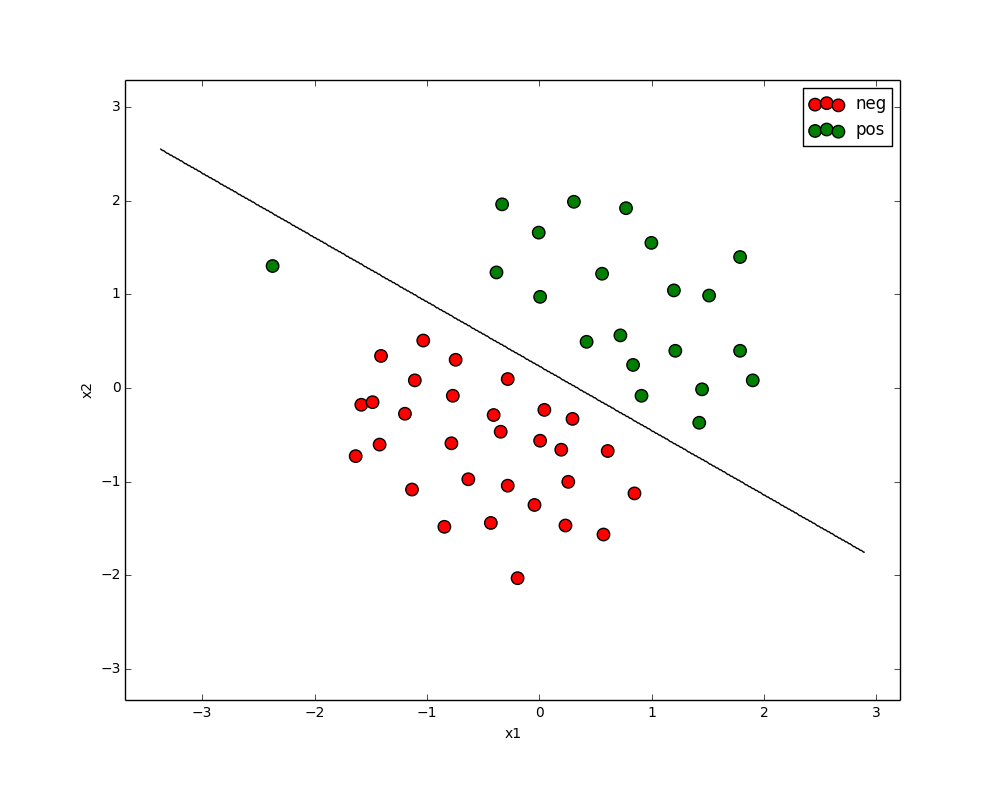
\includegraphics[scale=0.5]{c10.png}
\end{figure}

\begin{figure}[H]
  \caption{C=5}
  \centering
    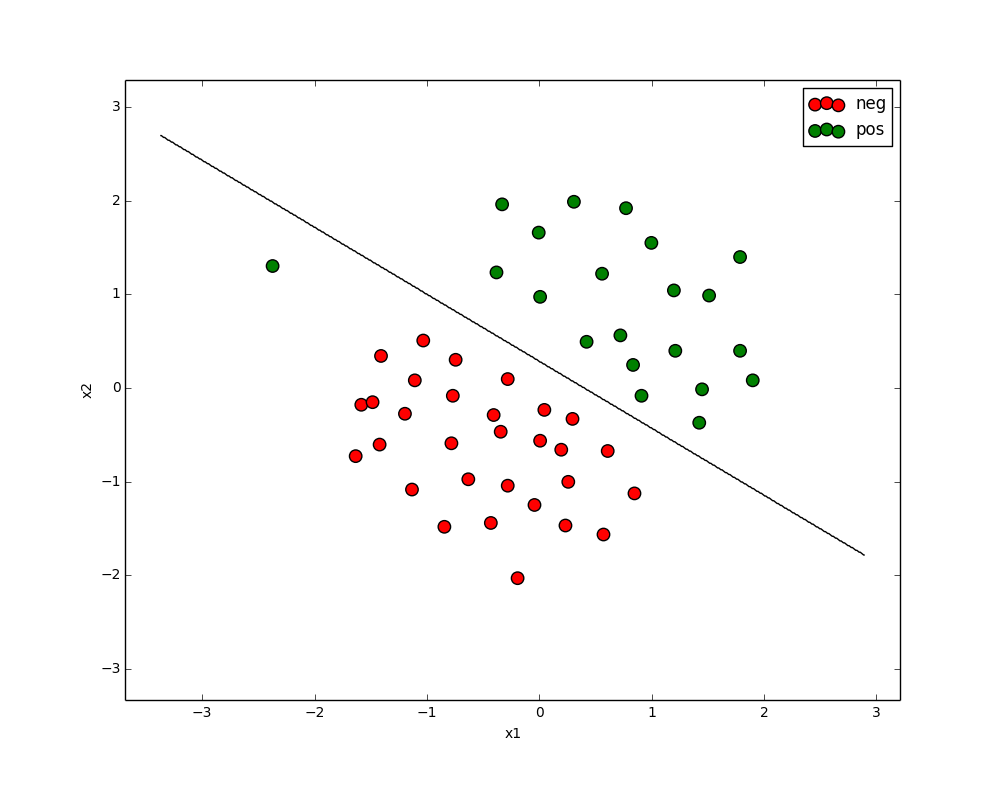
\includegraphics[scale=0.5]{c5.png}
\end{figure}





\subsection{Gaussian kernel}
\begin{lstlisting}


    k = 0
    k = np.exp(-np.linalg.norm(x1 - x2) ** 2 / (2 * sigma ** 2))
    return k
\end{lstlisting}
 And we get $Guassian kernel value (should be around 0.324652) =  0.324652467358$
 
 \begin{figure}[H]
  \caption{dataset2}
  \centering
    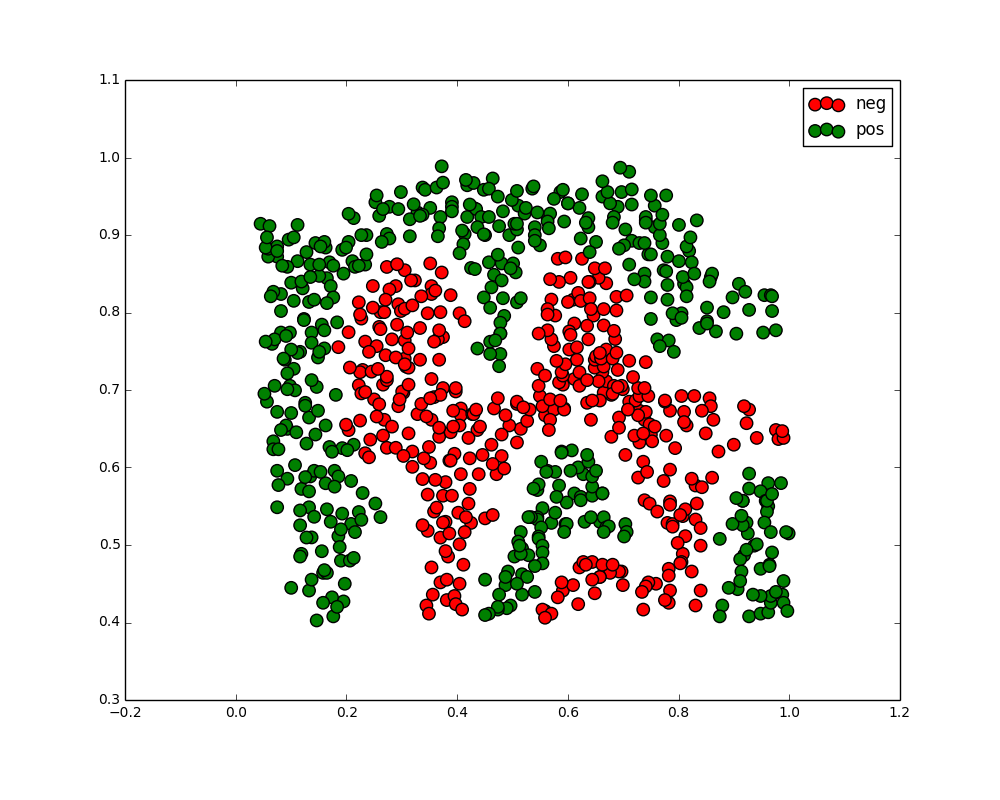
\includegraphics[scale=0.5]{dataset2.png}
\end{figure}

 \begin{figure}[H]
  \caption{sigma=0.01}
  \centering
    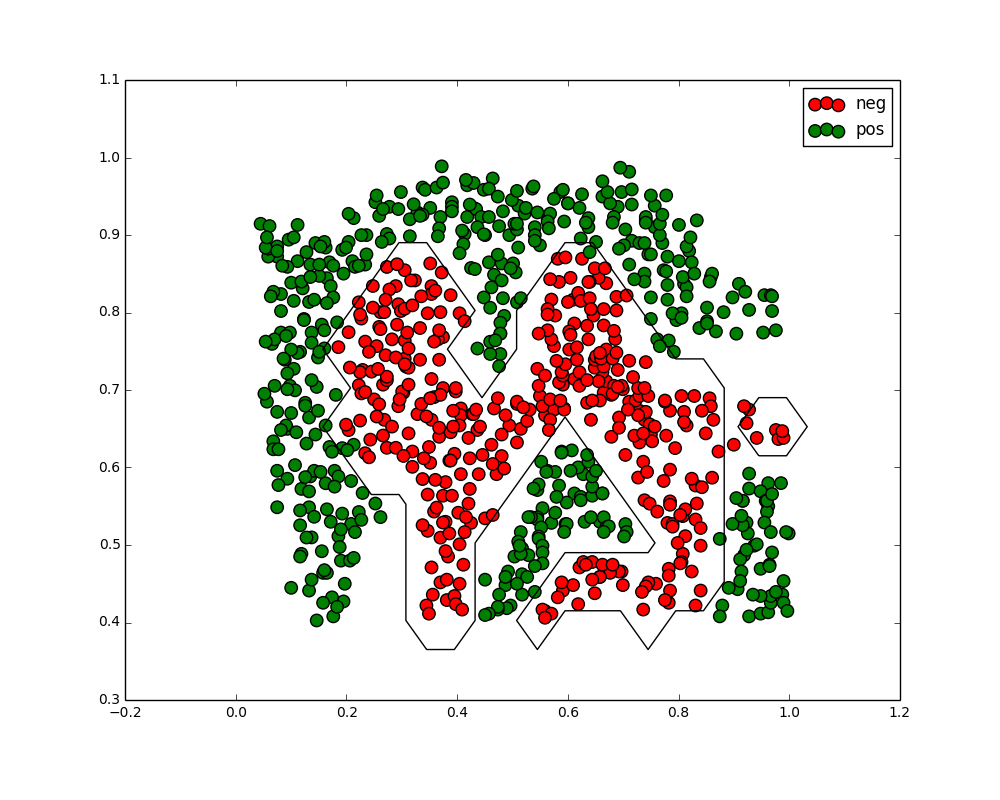
\includegraphics[scale=0.5]{sigma001.png}
\end{figure}
 

\subsection{selecting hyper parameters for SVM}
\begin{lstlisting}
best_acc = 0
svm = LinearSVM_twoclass()
for sigma in sigma_vals:
    K = np.array([utils.gaussian_kernel(x1, x2, sigma) for x1 in X for x2 in X]).reshape(X.shape[0], X.shape[0])
    scaler = preprocessing.StandardScaler().fit(K)
    scaleK = scaler.transform(K)
    KK = np.vstack([np.ones((scaleK.shape[0],)), scaleK]).T

    Kval = np.array([utils.gaussian_kernel(x1, x2, sigma) for x1 in Xval for x2 in X]).reshape(Xval.shape[0], X.shape[0])
    scalerval = preprocessing.StandardScaler().fit(Kval)
    scaleKval = scalerval.transform(Kval)
    KKval = np.vstack([np.ones((scaleKval.shape[0],)), scaleKval.T]).T

    for C in Cvals:
        svm.theta = np.zeros((KK.shape[1],))
        svm.train(KK, yy, learning_rate=1e-4, reg=C, num_iters=20000, verbose=False)
        yp = svm.predict(KKval)
        acc = metrics.accuracy_score(yyval, yp)
        print C, sigma, acc
        if acc > best_acc:
            best_acc = acc
            best_C = C
            best_sigma = sigma
print 'best', best_C, best_sigma, best_acc
\end{lstlisting}
I get the best c=0.1, best sigma=0.1

 \begin{figure}[H]
  \caption{best parameter,c=0.1,sigma=0.1}
  \centering
    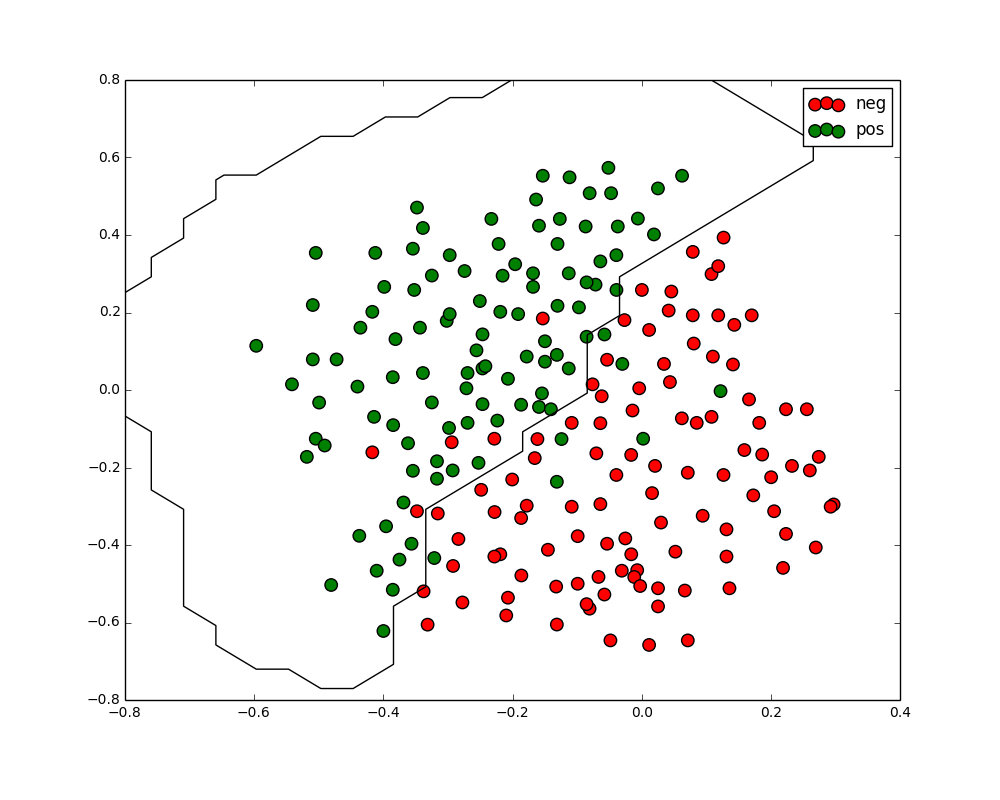
\includegraphics[scale=0.5]{0101.png}
\end{figure}

\subsection{Spam Classification with SVM}
\subsubsection{Training SVM for spam classfication}
Most values in Figure 10 is around 1000, except one value is 71,so I didn't scale the numbers. We chose no kernel, penalty parameter $C=0.1$, learning rate $\alpha=0.1$, and 10000 iterations. Here we add a cell to calculate the training accuracy. We had a 99.3\% training accuracy and a 99.1\% test accuracy. Our top 15 predictors of spam are listed below. At a cursory glance, most of these words do look like they belong in a spam email.\\
{\tt click, remov, our, basenumb, guarante, pleas, you, free, visit, here, nbsp,  will, hour,  most,dollar}\\
When choosing a kernel, we found that no kernel resulted in an average of 10\% increase in accuracy over a gaussian kernel. Because no kernel had an accuracy of over 98\%, we decided to simply use the raw features. We felt that there was no need for any kernelizing of the features due to this high accuracy.\\
In addition, we also saw an increase in accuracy if we didn't scale the data. We suspect this is because using the raw values put more weight onto words that appeared more frequently. Scaling was not really needed since counting the words caused them to be evaluated on the same scale already.\\
We ran our parameter sweep on three combinations of kernels/scaling. We found that (no kernel, no scaling) > (no kernel, scaling) > (kernel, scaling). This supported our decision to use no kernels and no scaling.\\
In sweeping our parameter space, we already knew that we were not going to use a kernel. So the only three parameters we had to sweep over was the penalty parameter, the learning rate, and the number of iterations. We ran across a number of combinations
$$C = [0.1, 0.3, 1, 3, 10, 30]$$
$$\alpha = [1e-2, 3e-2, 1e-1, 3e-1, 1, 3]$$
and found the best accuracy on our 20\% validation split was for $C=0.1$ and $\alpha=0.1$. The loss plateaued around 7500 iterations, so we found that 10000 iterations was more than enough. Given our 99\%+ accuracy on both training and test data, we are satisfied with our results.

\section{Support vector machines for multi-class classification}
\subsection{5A naive version}

\begin{lstlisting}
  K = theta.shape[1]
  m = X.shape[0]
  dtheta = np.zeros(theta.shape)
  J = 0.0
  for i in xrange(m):
    scores = X[i,:].dot(theta)
    correct_class_score = scores[y[i]]
    for j in xrange(K):
      if j == y[i]:
        continue
      margin = max(0,scores[j] - correct_class_score + delta)
      #J += margin
      if margin > 0:
        J += margin
        dtheta[:,j] += X[i]
        dtheta[:,y[i]] -= X[i] 
        
          J /= m
  dtheta /=m
  # Add regularization to the loss.
  J += 0.5 * reg * np.sum(theta * theta)/m

  dtheta +=reg*theta/m
        
\end{lstlisting}
\subsection{5B, vector version}
\begin{lstlisting}
J = 0.0
  dtheta = np.zeros(theta.shape) # initialize the gradient as zero
  delta = 1.0
  num_classes = theta.shape[1]
  num_train = X.shape[0]
  scores = X.dot(theta)
  Y = np.zeros(scores.shape)
  for i,row in enumerate(Y):
    row[y[i]] = 1
  
  Correct_class_scores = np.array( [ [ scores[i][y[i]] ]*num_classes for i in range(num_train) ] )  
  Margin = scores - Correct_class_scores + ((scores - Correct_class_scores) != 0)*delta
  X_with_margin_count = np.multiply(X.T , ( Margin > 0).sum(1) ).T

  J += np.sum((Margin>0)*Margin)/num_train
  J += 0.5 * reg * np.sum(theta * theta)/num_train
  dtheta += ( Margin > 0 ).T.dot(X).T/num_train
  dtheta -= (Margin == 0).T.dot(X_with_margin_count).T/num_train
  dtheta += reg*theta
\end{lstlisting}
It takes 1206.436000s.
\subsection{5c Prediction function}
\begin{lstlisting}
    Scores = X.dot(self.theta)
    y_pred = np.argmax(Scores, axis = 1)
\end{lstlisting}

we get training accuracy 0.361245 and validation accuracy 0.362000

\subsection{5D tning hyper parameters}
I get an validation accuracy of 0.406000 with learning rate of 1e-6 and reg 1e4.The code is here:
\begin{lstlisting}
for learning_rate in learning_rates:
    for reg in regularization_strengths:
        print("LR",learning_rate,"reg",reg)
        svm = LinearSVM()
        loss_hist = svm.train(X_train, y_train, learning_rate, reg,
                      num_iters=1500, verbose=True)
        y_train_pred = svm.predict(X_train)
        y_val_pred = svm.predict(X_val)
        results[(learning_rate,reg)] = (np.mean(y_train == y_train_pred),np.mean(y_val == y_val_pred))
        
        if best_val < np.mean(y_val == y_val_pred):
            best_val = np.mean(y_val == y_val_pred)
            best_parameters = { 'LR':learning_rate, 'reg': reg}




\end{lstlisting}

\subsection{5E }
 \begin{figure}[H]
  \caption{accuracy}
  \centering
    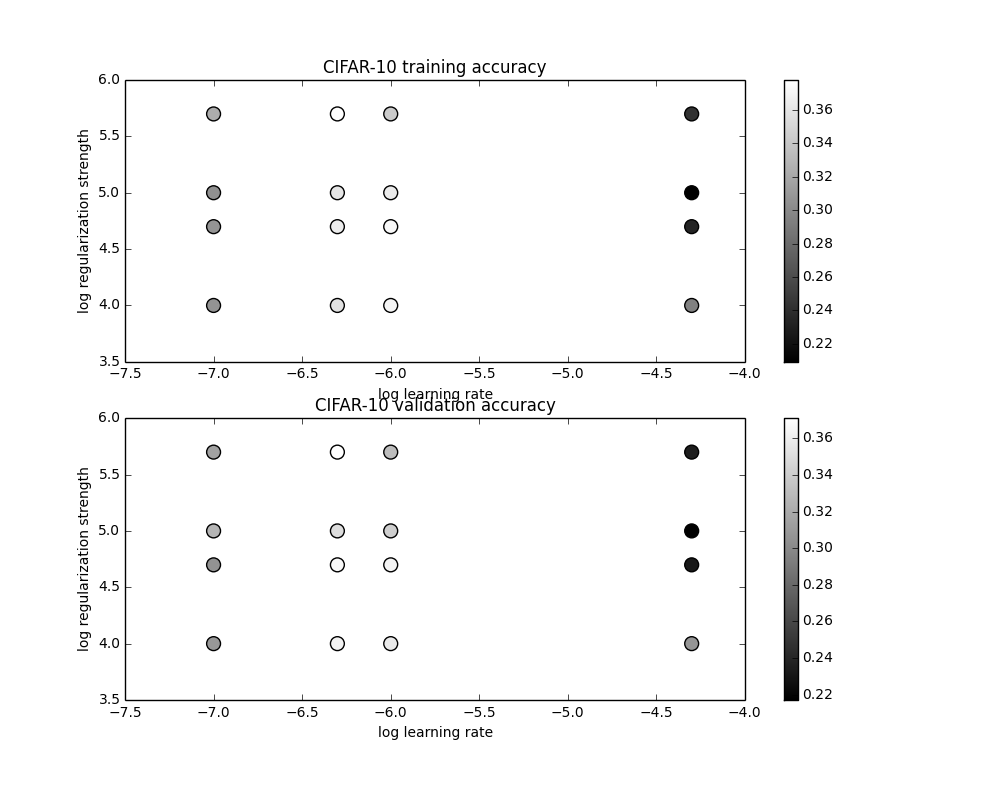
\includegraphics[scale=0.5]{visz.png}
\end{figure}
The SVM takes longer time. And for the accuracy, Softmatrix is slightly better . It is 0.403 better than 0.369.As for the theta I still think Softmatrix is better.As for the running time, I think softmatrix is better. 
The SVM has a test accuracy of 0.369.
\begin{figure}[H]
  \caption{hw3}
  \centering
    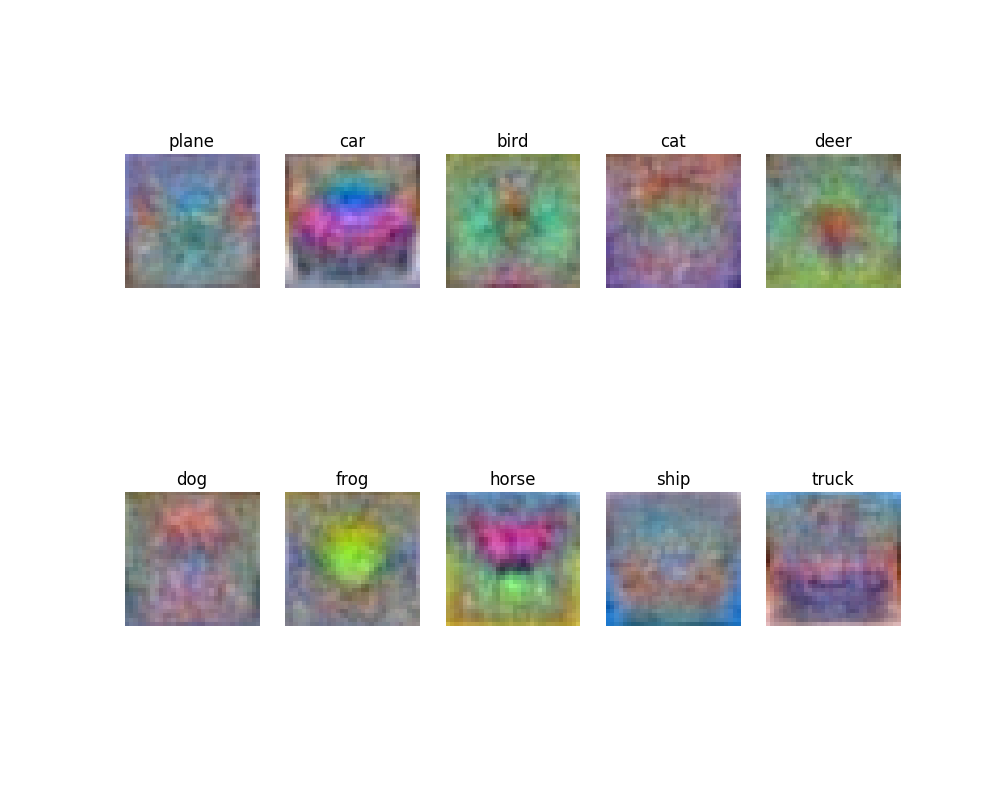
\includegraphics[scale=0.5]{classifernew.png}
\end{figure}

\begin{figure}[H]
  \caption{hw4}
  \centering
    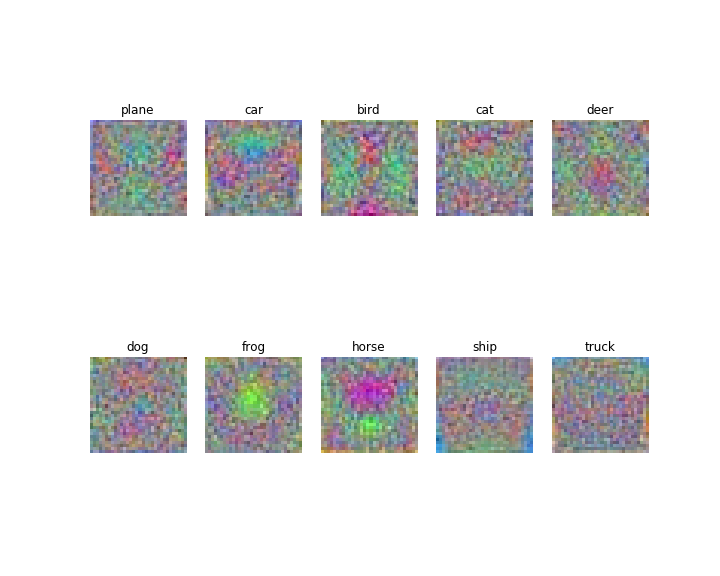
\includegraphics[scale=0.5]{hw4fe.png}
\end{figure}










 



\end{document}
